\documentclass[10pt]{article}
\usepackage[utf8]{inputenc}

\usepackage{geometry}
\geometry{a4paper}

\usepackage{fancyhdr}
\usepackage{calc}
\usepackage{multirow}
\usepackage[explicit]{titlesec}
\usepackage{graphicx}
\graphicspath{ {images/}{/home/ernesto/.TeXworks/templates/Custom_templates/} }
\usepackage{xcolor}
\usepackage[hidelinks]{hyperref}

\newlength{\w}
\setlength{\w}{\textwidth / 5 - 1.18pt}

\newcommand*\getlength[1]{\number#1}

\pagestyle{fancy}
\fancyhf{}
\rhead{\textit{Grupo Scout 109 Monte Clavijo} \\}
\lhead{Campamento de Verano 2017 \\ Zarzosa (La Rioja)}
\cfoot{
\includegraphics[width=\getlength{\w}sp]{logo}
	
\includegraphics[width=\getlength{\w}sp]{logo}
\includegraphics[width=\getlength{\w}sp]{logo}
	
\includegraphics[width=\getlength{\w}sp]{logo}
\includegraphics[width=\getlength{\w}sp]{logo}}

\titleformat{\section}
  {\Large\bfseries}{\thesection}{5em}{#1}[{\titlerule}]

\begin{document}
\large
\fontencoding{T1}\fontfamily{lmss}\fontseries{m}\fontshape{n}\selectfont
\begin{tabular}{|p{2cm}|c|}
\hline
\multirow{5}{*}{
\includegraphics[width=2cm]{logo}} & \textbf{CLAN} \\
\cline{2-2}
& \textbf{BOMBA DE ARIETE} \\
\cline{2-2}
& \parbox{\textwidth-4cm}{Fecha y momento del dia: \textbf{16 jullio - tarde}} \\ %Fecha
& \parbox{\textwidth-4cm}{Duracion: \textbf{1.5 horas}} \\ %Duracion
& \parbox{\textwidth-4cm}{Destinatarios/as: \textbf{jovenes de 17 a 21 años}} \\ %Destinatarios
\hline
\end{tabular}

\section*{DESCRIPCI\'ON}
Se realizar\'a una bomba de ariete que (si sale bien), servir\'a como sustituto a la actual
motobomba que se usa en el campamento, de tal manera que no se har\'a tanto ruido
y no se gastar\'a gasolina.

\section{OBJETIVOS}
\begin{itemize}
\item Realizar una bomba de ariete y prestar as\'i un servicio al grupo.
\end{itemize}

\section{DESARROLLO}
Se montan las piezas tal y como se muestra en la figura:
\begin{center}
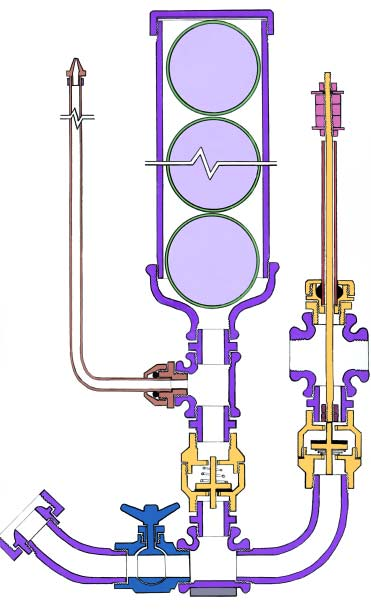
\includegraphics[width=6.5cm]{images/bomba-de-ariete}
\end{center}
Una vez montada, se divide al clan en 2. Unos ir\'an a instalar la alimentaci\'on y la salida de la
bomba, mientras otros la calibran.
\par
Para calibrar la bomba, se necesita que est\'e alimentada (lo cual se puede conseguir
temporalmente con un balde de agua puesto en altura), una vez abierta la llave de paso,
se ajusta el peso de la varilla de cobre hasta que la bomba empieze a funcionar. Si se quiere
un mejor rendimiento, se puede seguir modificando el peso de la varilla m\'aximizando el tiempo
que dura cada ciclo (el tiempo que pasa desde que se cierra la v\'alvula antiretorno hasta que se
vuelve a cerrar).
\par
Para la instalaci\'on, se necesita una fuente de agua (el r\'io del campamento), desde donde se
enviar\'a el agua mediante un tubo hacia la bomba. El tubo de alimentaci\'on de la bomba ha
de estar lo m\'as recto posible (se puede atar a una madera, o un palo recto) y debe tener una
inclinaci\'on de entre 10 y 45 grados. Una vez colocado el tubo de alimentaci\'on, se mueve la
bomba a su posici\'on definitiva y se conecta el tubo de salida a los bidones.
\section{MATERIALES}
\begin{itemize}
\item Los necesarios para la bomba de ariete (Especificados en las p\'aginas 6 y 7 del pdf
{\color{blue}\url{http://www.terra.org/data/ariete_super.pdf}})
\item Tefl\'on para sellar las juntas
\item Ser\'an utiles llaves de fontanero grandes para apretar bien las juntas (aunque son
prescindibles ya que esta bomba es temporal)
\end{itemize}
\section{SUGERENCIAS}
\begin{itemize}
\item en el montaje, se puede dividir al clan en dos grupos, unos montan el cuerpo de la bomba,
y otros montan el ariete
\item Se puede acabar de calibrar la bomba una vez colocada en su emplazamiento final, para
conseguir una mejor eficiencia
\item Cuanta m\'as altura haya entre la fuente de agua y la bomba, mejor funcionar\'a
\end{itemize}
\section{EVALUACION}
\begin{itemize}
\item ¿Han construido una bomba de ariete funcional?
\item ¿Saben como instalarla para pr\'oximos campamentos?
\end{itemize}
\section{FUENTE}
G. S. 109 Monte Clavijo
\\
{\color{blue} \url{http://www.terra.org/}}
\end{document}
